\documentclass[tikz, border=2pt]{standalone}

\usepackage{helvet}
\renewcommand{\familydefault}{\sfdefault}

\usepackage[EULERGREEK]{sansmath}
\sansmath
\usetikzlibrary{arrows.meta}

\begin{document}%

\begin{tikzpicture}[line width=2pt]
\tikzset{>={Latex[width=3mm,length=4mm]}}

% % grid
% \draw[help lines] (-0.5, -5) grid (13, 18);

  \node[inner sep=0pt] (figa) at (5,10.5)
  {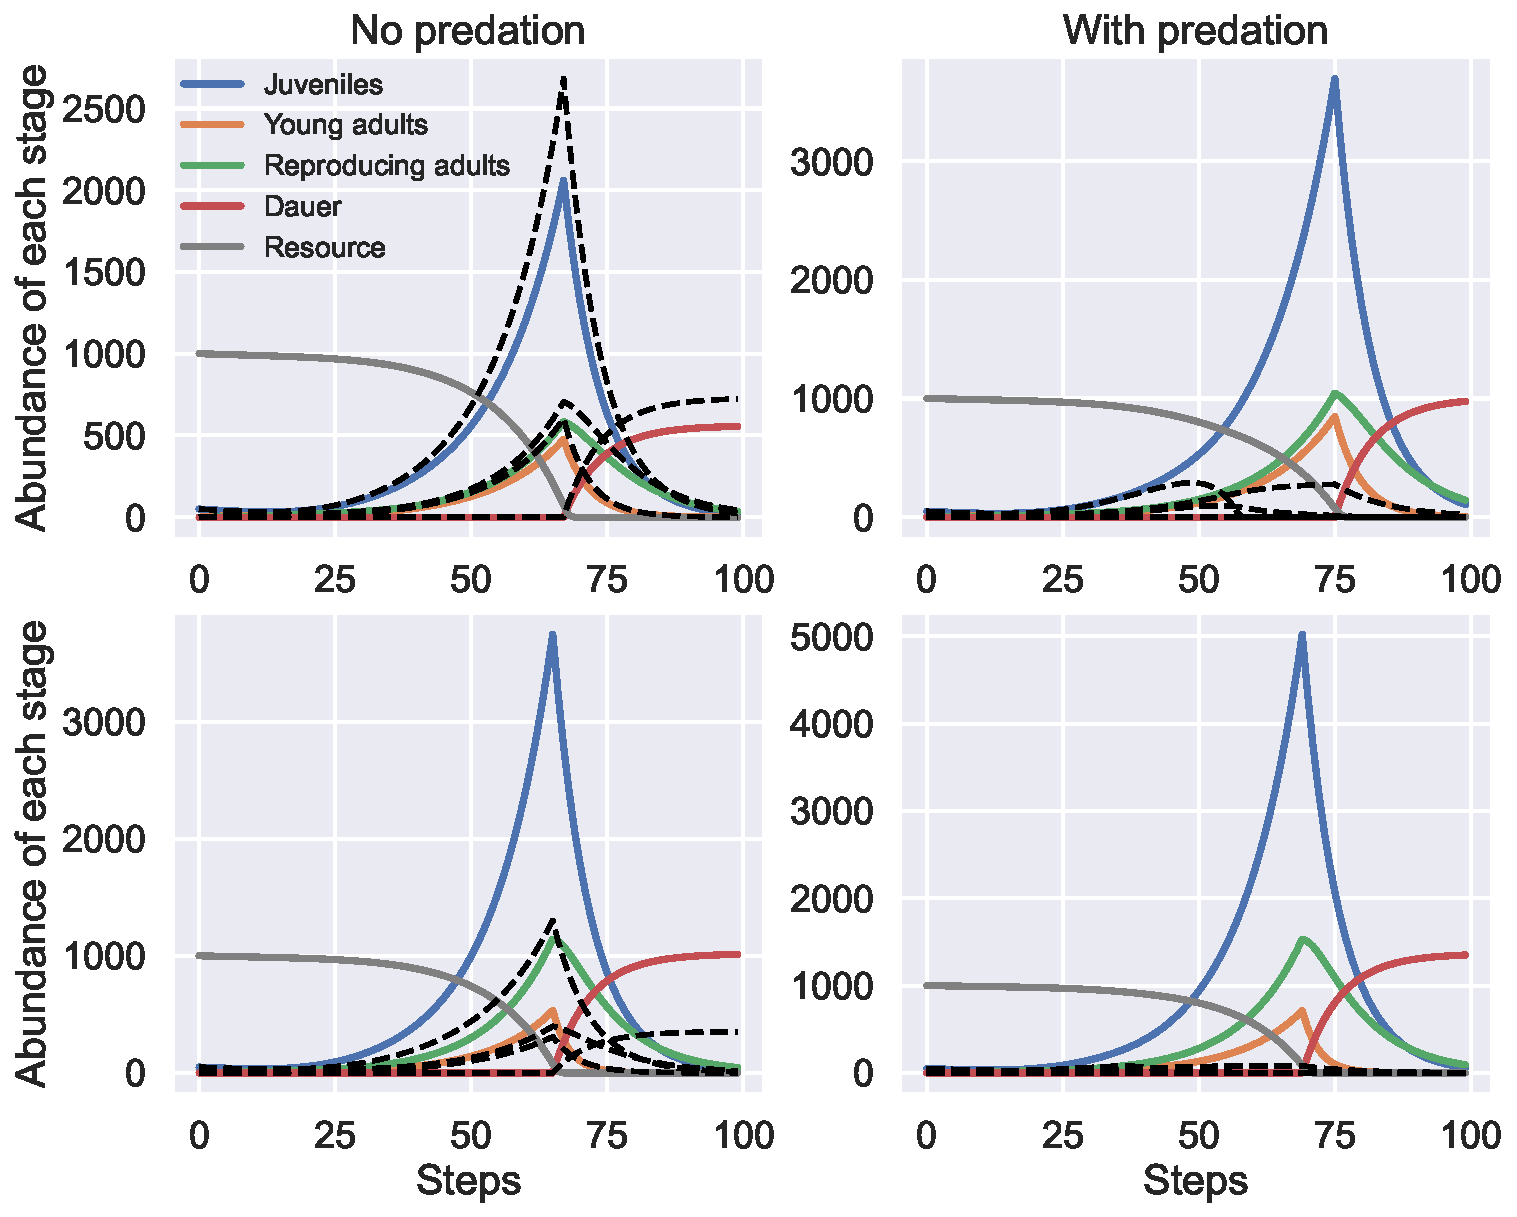
\includegraphics[width=0.8\textwidth]{PopDynamic_with_interaction.pdf}};


  \node[inner sep=0pt] (figa) at (11.3,8.7)
  {
\includegraphics[width=0.15\textwidth]{../diffusion.pdf}};

  \node[inner sep=0pt] (figa) at (13.3,8.7)
  {
\includegraphics[width=0.15\textwidth]{../diffusion_2.pdf}};

  \node[inner sep=0pt] (figa) at (12.3,12.5)
  {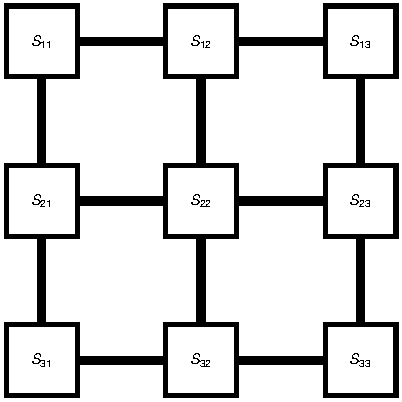
\includegraphics[width=0.3\textwidth]{./tikz_figs/meta_pop.pdf}};

  \node[inner sep=0pt] (figa) at (2,2.5)
  {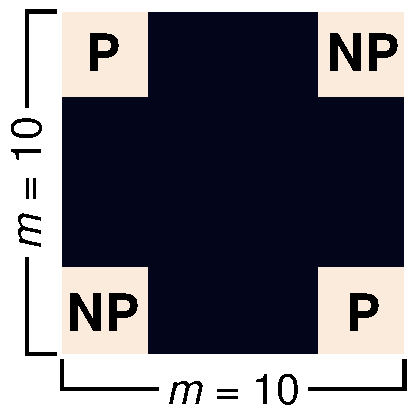
\includegraphics[width=0.3\textwidth]{./tikz_figs/pop_icon.pdf}};

  \node[inner sep=0pt] (figa) at (9.5,2.5)
  {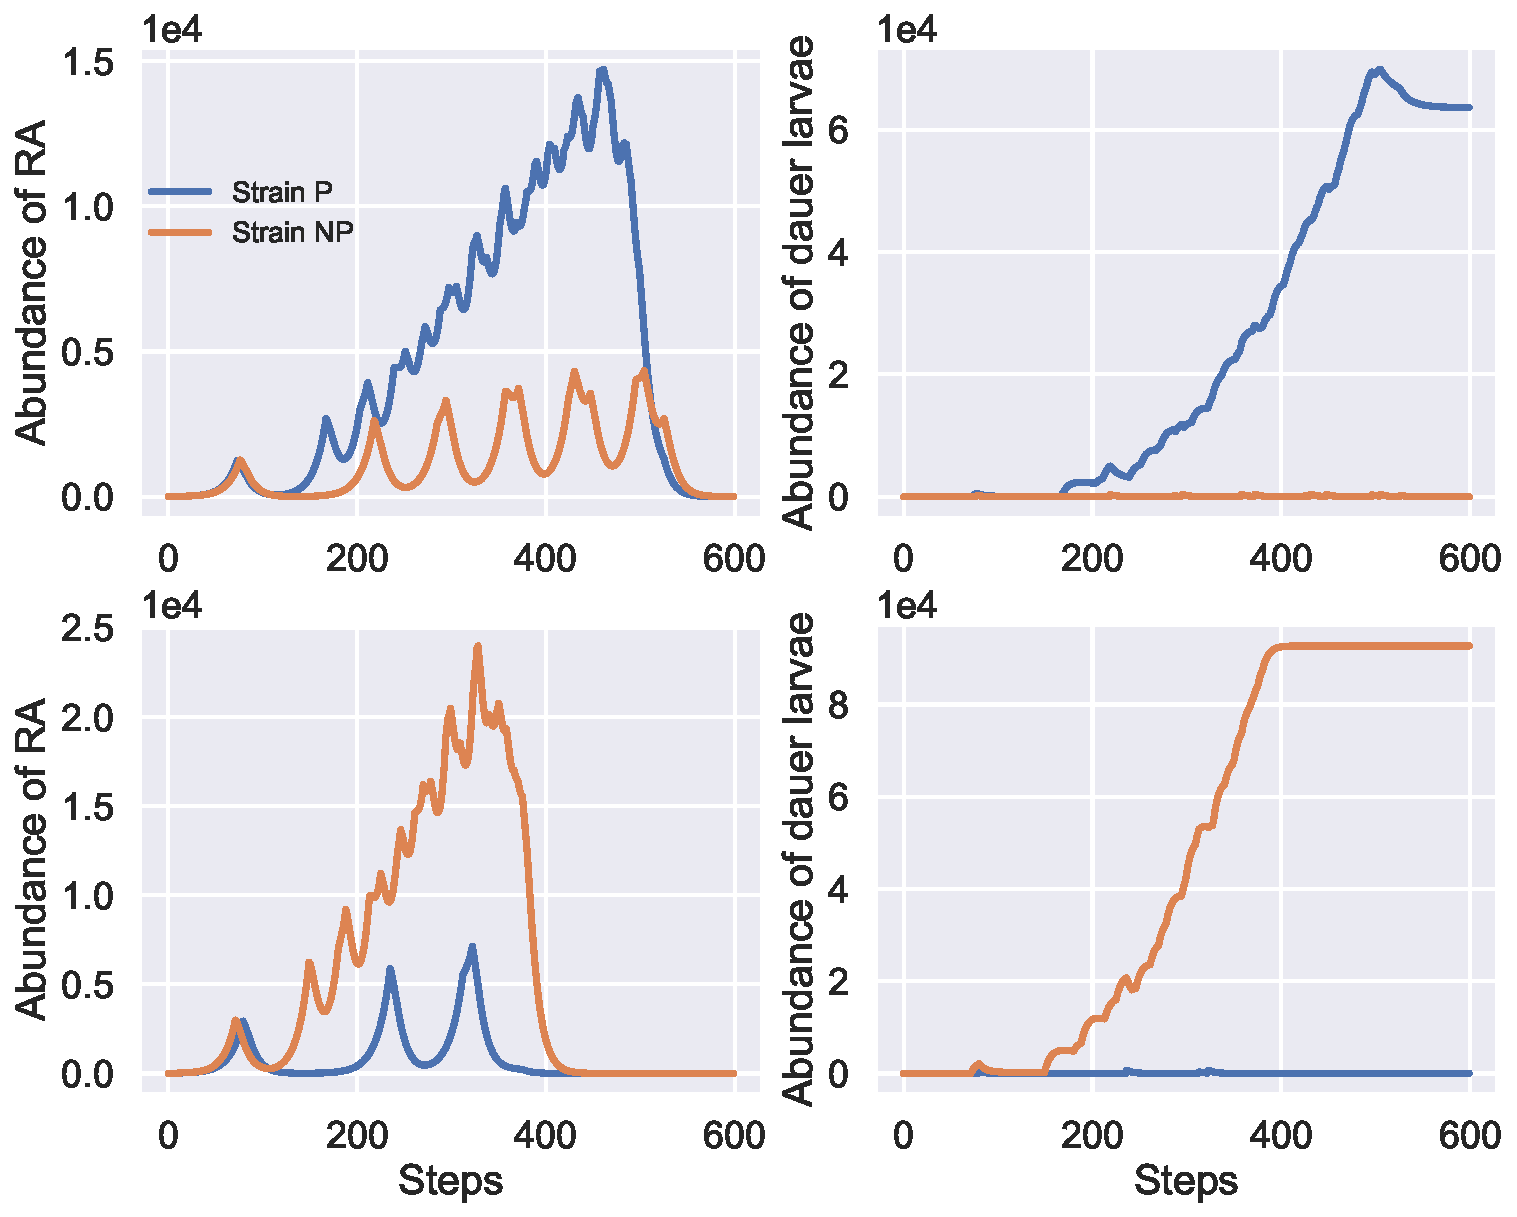
\includegraphics[width=0.77\textwidth]{../meta_uniform.pdf}};

\node at (-0.1,12.5) [draw=none, rectangle, fill=black!20,rotate=90] (g1) {\sf \small \emph{E. coli} OP50};

\node at (-0.1,9) [draw=none, rectangle, fill=black!20, rotate=90] (g1) {\sf \small \emph{Novosphingobium}};

\node at (4.5,4.4) [draw=none, rectangle, fill=black!20,rotate=90] (g1) {\sf \small \emph{E. coli} OP50};

\node at (4.5,1) [draw=none, rectangle, fill=black!20, rotate=90] (g1) {\sf \small \emph{Novosphingobium}};


\node at (11.4,7.5) [draw=none, rectangle, rotate=0] (g1) {\sf \large $\tau_1$};
\node at (13.4,7.5) [draw=none, rectangle, rotate=0] (g1) {\sf \large $\tau_2$};
%labels
\draw (0., 14.8) node{{\Huge\sf\textbf{a}}};

\draw (10.3, 14.8) node{{\Huge\sf\textbf{b}}};

\draw (10.3, 10.3) node{{\Huge\sf\textbf{c}}};

\draw (0., 6.3) node{{\Huge\sf\textbf{d}}};

% \draw (0., 11.5) node{{\Huge\sf\textbf{c}}};

% \draw (0., 6.3) node{{\Huge\sf\textbf{d}}};


\end{tikzpicture}


\end{document}